ATLAS is a general-purpose particle detector

% brief overview of detector
% define coordinate system, eta, DeltaR

\begin{figure}[tbp]
  \begin{center}
    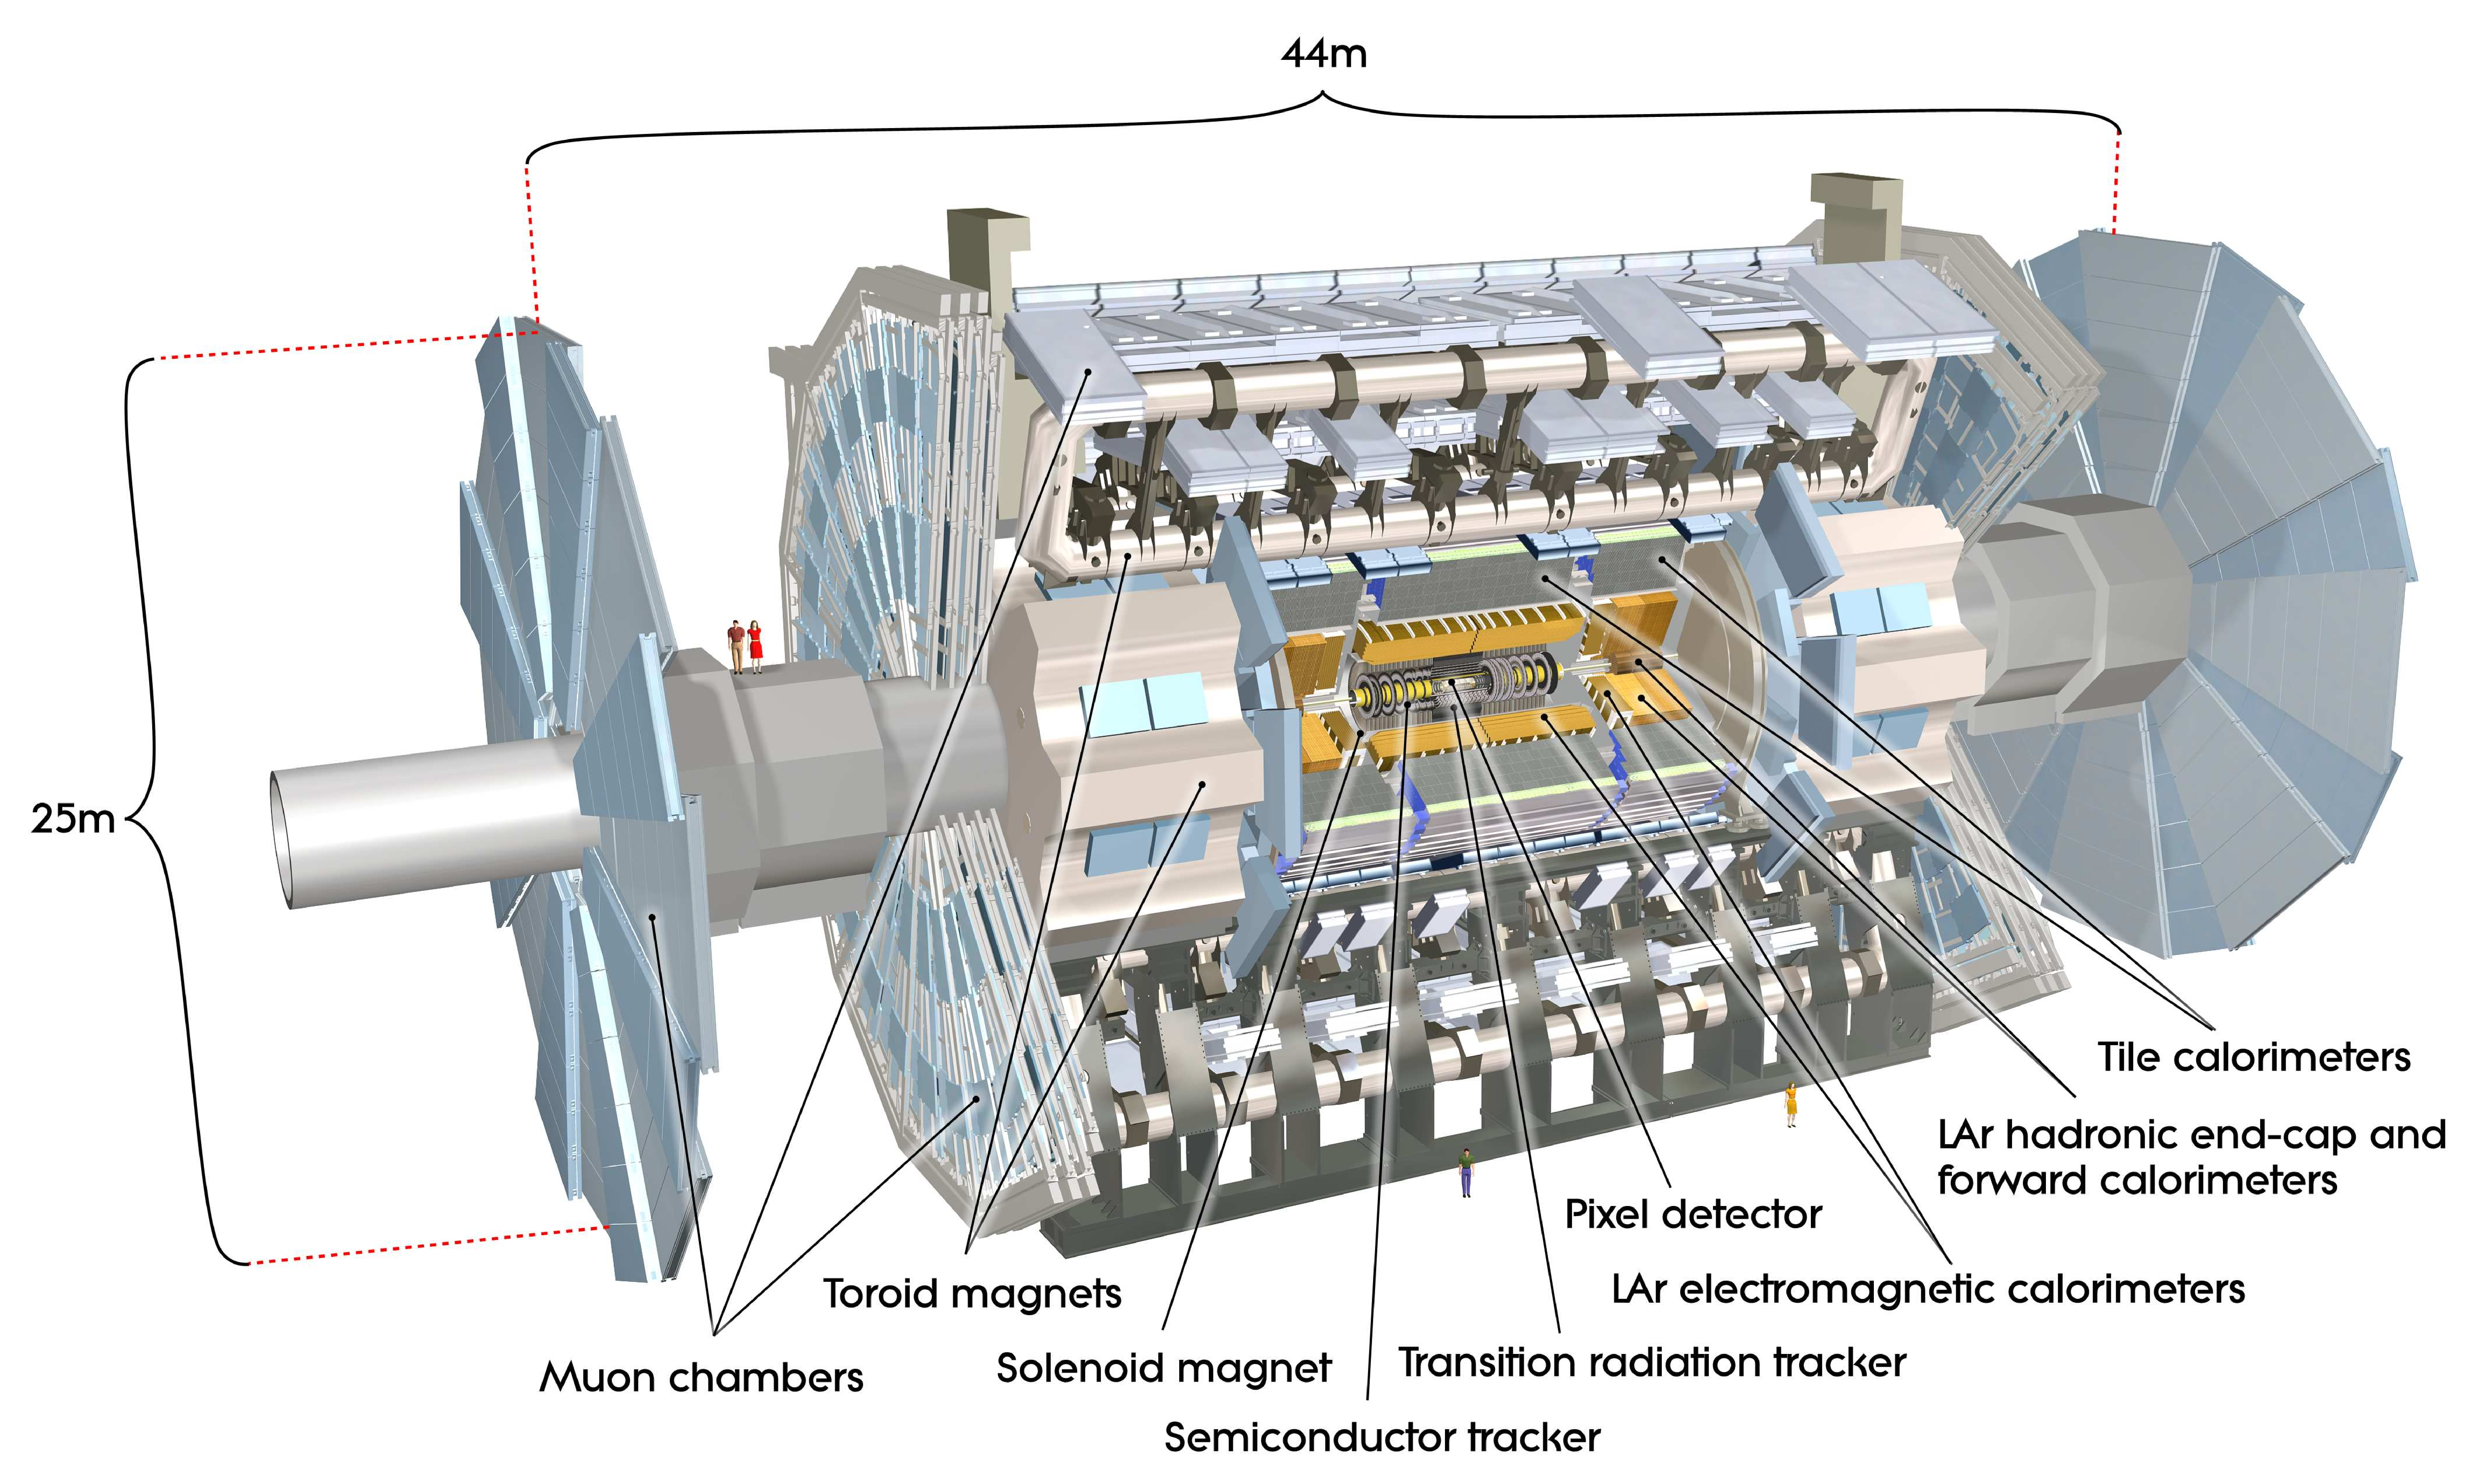
\includegraphics[width=0.98\textwidth]{figs/detector/atlas.pdf}
  \end{center}
  % Optional first argument is what goes into the List of Figures, useful if main caption is long or contains references
  % Second argument here is the actual caption
  \caption[General cut-away view of the ATLAS detector.]
          {General cut-away view of the ATLAS detector \cite{PERF-2007-01}.}
\end{figure}
